% multiple1902 <multiple1902@gmail.com>
% intro.tex
% Copyright 2011~2012, multiple1902 (Weisi Dai)
% https://code.google.com/p/xjtuthesis/
%
% It is strongly recommended that you read documentations located at
%   http://code.google.com/p/xjtuthesis/wiki/Landing?tm=6
% in advance of your compilation if you have not read them before.
%
% This work may be distributed and/or modified under the
% conditions of the LaTeX Project Public License, either version 1.3
% of this license or (at your option) any later version.
% The latest version of this license is in
%   http://www.latex-project.org/lppl.txt
% and version 1.3 or later is part of all distributions of LaTeX
% version 2005/12/01 or later.
%
% This work has the LPPL maintenance status `maintained'。
%
% The Current Maintainer of this work is Weisi Dai。
%

\chapter{基于显著性图的缺陷检测算法}
\echapter{Saliency based Defect Detection Method}
图像显著性提取即将图像中视觉最突出的部分与其他区域划分开来,自从1998年Itti \cite{Itti1998A} 的工作以来,产生了大量的显著性映射方法\cite{Zhai2006Visual, Cheng2011Global, Achanta2008Salient, Achanta2009Frequency},图像显著性也广泛应用于图像压缩、编码、图像边缘和区域加强、显著性目标分割和提取等。使用显著性处理钢板表面的缺陷的基本原理是通过显著性方法对图像进行预处理,达到更好的突出缺陷区域的目的,并结合边缘检测等手段,最终将缺陷部分提取出来。
    \section{方法概述}
    \esection{Outline}
    由于生产条件和图像采集等诸多因素的影响,导致目前基于机器视觉的检测存在很多技术难点,如低对比度、图像质量过差、各类伪缺陷等。因此,本章提出了一种基于显著性的检测方法。

    基于显著性的缺陷检测方法先对输入的钢板图像进行显著性图的提取,通过这个步骤进行图像对比度的提升以及噪声的滤除,接着利用多个的显著性图所包含图像信息之间的差异去除黑斑,在这个步骤里同时使用了canny边缘检测\cite{Canny1986A}手段提取出缺陷区域的具体位置,当得到去除黑斑的边缘结果之后通过形态学膨胀将相邻的缺陷区域进行融合,最后进行缺陷的标注工作,具体流程如图\ref{fig:c3_flow_chart} 所示。

    \begin{figure*}[!h]
    \centering
    
\includegraphics[width=16cm]{c3_flow_chart.png}
    \caption{基于显著性的缺陷检测算法流程图}
    \label{fig:c3_flow_chart}
    \end{figure*}

    \section{显著性检测}
    \esection{Saliency Map Detection}
        \subsection{基于显著性图的对比度提升}
        \esubsection{Saliency Map based Contrast Enhancement}
        首先使用FT显著性检测方法\cite{Achanta2009Frequency}来处理钢板缺陷,主要因为该方法简单快速,符合缺陷检测的实时性要求,并且该方法能够显著提高缺陷区域与背景区域的对比度,对缺陷识别有很好的效果。

        该方法主要原理是通过使用两个高斯滤波器完成对图像不同频段的滤波操作,在实现上通过求取图像均值以及高斯滤波图像的距离完成显著性图的生成。具体来说,对于一幅输入图像,分别进行$lab$ 空间的均值操作以及高斯滤波操作,再通过公式( \ref{equ:c3_salient} )求取两幅图像对应位置的欧式距离就可以得到最终的显著性图。公式中$I_\mu$ 表示图像均值, $I_{whc}\left( {x, y} \right)$ 表示在$\left( {x, y} \right)$坐标位置的高斯滤波后的像素值。
        \begin{eqnarray}
        S\left( {x,y} \right) = \left\| {I_\mu - I_{whc}\left( {x, y}\right)} \right\|
        \label{equ:c3_salient}
        \end{eqnarray}
        针对本文中所提到的低对比度缺陷,该方法有很好的对比度提升效果,如图\ref{fig:c3_salient}所示,其中从左至右分别为原图、原图的边缘检测结果、显著性图、对显著性图做边缘检测的结果。对比直接使用原图进行边缘检测的结果我们发现使用显著性处理之后的图像检测到的边缘更加完整,噪声更少,但是在这里有必要说明的一点是提取显著性图时并非直接使用公式,而是使用了改进的显著性检测,这部分内容将会在接下来的章节详细讲述。

        \begin{figure*}[!h]
        \centering
        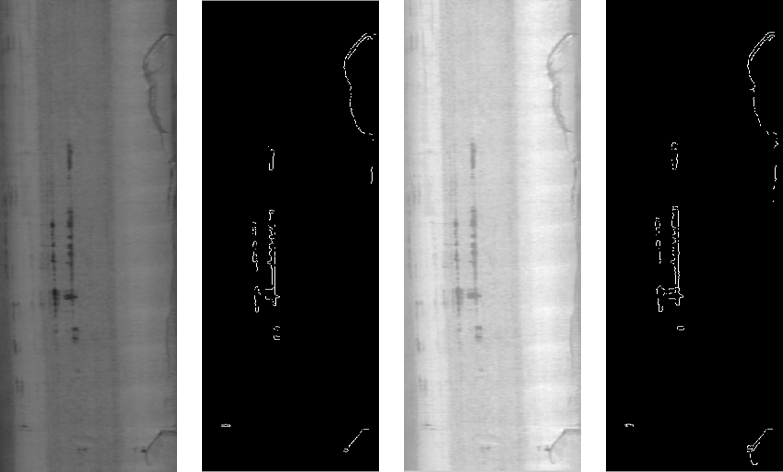
\includegraphics[width=16cm]{c3_salient.png}
        \caption{显著性检测对缺陷检测的提升效果}
        \label{fig:c3_salient}
        \end{figure*}

        \subsection{改进的显著性检测}
        \esubsection{Improved Saliency based Detection}
        上述提到的检测中,黑斑部分也作为一部分缺陷进行了检测,但是实际生产过程中,黑斑是作为一种伪缺陷并不需要进行检测,本节将使用一种改进的显著性检测方法去除这种伪缺陷对检测结果的干扰。

        公式中的$I_\mu$代表图像的均值,很显然在一副图像中大面积的背景区域对于图像的均值起着决定性的作用,这也是为什么直接使用公式对图像进行处理时如图\ref{fig:c3_multi_salient}中$\lambda = 1$的情况,背景区域将会变为全黑,基于此我们做一个变形:
        \begin{eqnarray}
        S\left( {x, y} \right) = \left| {\lambda * I_\mu - I_{whc}\left( {x, y}\right)} \right|, \lambda \in \left[ {0, 1} \right]
        \end{eqnarray}
        通过调整$\lambda$的取值,我们可以得到不同的显著性图,如图\ref{fig:c3_multi_salient}所示,当$\lambda$取值不同时,我们可以认为人为改变了图像的”背景“,相对应的”前景“区域也发生了变化,根据这种特点,我们可以容易得到图像中不同层次的内容,也就可以将黑斑的区域从图像中剔除出来。

        \begin{figure*}[!h]
        \centering
        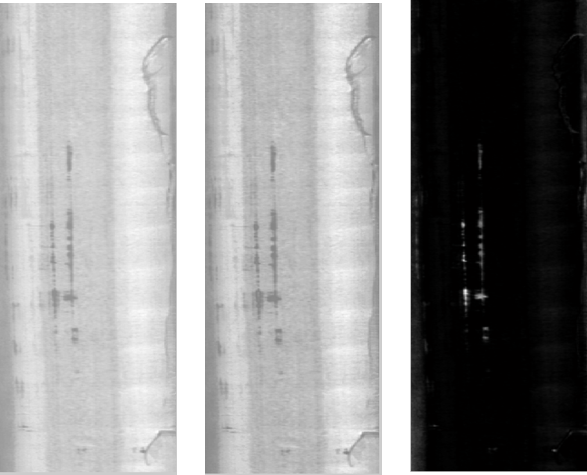
\includegraphics[width=16cm]{c3_multi_salient.png}
        \caption{使用不同$\lambda$的显著性检测效果,从左至右分别为$\lambda = 0.3$、$\lambda = 0.5$和$\lambda = 1$}
        \label{fig:c3_multi_salient}
        \end{figure*}

        对于一幅输入图像,分别对图像使用两个$\lambda$ 取值不同的显著性提取,一方面设$\lambda$为0.5得到同时包含缺陷和黑斑并且对比度进行加强的图像,接着对显著性图像进行canny边缘提取,得到备用的缺陷图像;另一方面使用$\lambda$ 为1进行显著性提取,使得图像只包含最显著的目标,即黑斑区域(实际上在一幅图像里,黑斑区域较其他区域具有明显的显著性目标特征),针对这幅图像,我们使用一个简单的二值化操作将黑斑的区域提取出来,由于可能检测到的黑斑区域并不十分完整,因此采取形态学膨胀的手段使得黑斑包围的面积更加完全,即使超出了原有黑斑的区域,在接下来的减除操作里,也可以避免这种误差造成的影响。在得到了上述两幅图像之后,进行作差工作,具体的原理如公式( \ref{equ:c3_black_spot_1} ) ( \ref{equ:c3_black_spot_2} ) 所示,$I_e$ 表示边缘检测的结果,$I_b$ 表示二值化和膨胀后的结果,作差后的结果$I_m$ 即为去黑斑后的中间结果图像。
        \begin{eqnarray}
        I_m = \Delta \left( {I_e - I_b} \right)
        \label{equ:c3_black_spot_1}
        \end{eqnarray}
        其中,函数$\Delta$为阶跃函数,其函数形式为:
        \begin{eqnarray}
        \Delta \left( x \right) = \left\{ \begin{matrix}
        0,&x<=0\\
        1,&x>0
        \end{matrix}\right.
        \label{equ:c3_black_spot_2}
        \end{eqnarray}
    \section{边缘提取}
    \esection{Edge Detection}
    在获得显著性图像之后,对图像进行边缘提取获得边缘图像。图像边缘是指邻域内像素的灰度值存在较大变化的像素点的集合,在频域上表示了图像的高频区域,在灰度图像上反映出了图像中灰度值的不连续性。图像的边缘检测\cite{Gonzalez2010Digital}能够大幅减少数据量,并且剔除不相关信息,保留图像中最重要的结构信息。边缘检测的实际目标是利用某种算法来提取图像中目标与背景之间的边缘线,通常可以由图像的一阶导数的最大值或者二阶导数的过零点检测得到图像边缘。常用的一阶导数有Roberts、Prewitt、Sobel 等\cite{Heath1998Comparison}梯度算子;基于二阶导数过零点检测的边缘检测算子中最典型的是由 Marr等提出的LoG算子\cite{Gonzalez2010Digital}。这些检测方法都是基于局部滑动窗的方法,其检测效果一般不理想,检测出的边缘并不完整存在断裂情况,并且往往会产生较多噪声。

    该方法使用Canny边缘检测算法\cite{Canny1986A}来提取边缘图像,相比较于其他的边缘检测算子,Canny算子具有较大的信噪比和较高的检测精度。Canny边缘检测算法的目标是找到一个最优的边缘检测算法,其认为最优边缘检测的目标是:

    1)最优的检测:即算法能够尽可能多的找出图像中的实际边缘;

    2)最优的定位:即算法标识出的边缘要尽可能与图像中的边缘位置一致;

    3)最小的响应:即图像中的边缘应最多被标识一次,并且尽可能减少噪声的误检情况:

    Canny边缘检测方法的一般步骤如下所示:

    1)计算图像与高斯平滑滤波器的卷积结果;

    2)使用一阶梯度算子计算图像的水平方向梯度图和垂直方向梯度图;

    3)根据水平方向梯度图和垂直方向梯度图计算梯度幅值和方向;

    4)使用非极大值抑制,细化梯度图像,只保留梯度幅值变化最大的那个点。

    使用Canny边缘检测方法在显著性图像上提取边缘来获取缺陷候选项,Canny边缘检测的效果如图所示,从左至右依次为原图、显著性图像、边缘图像。

    \begin{figure*}[!h]
    \centering
    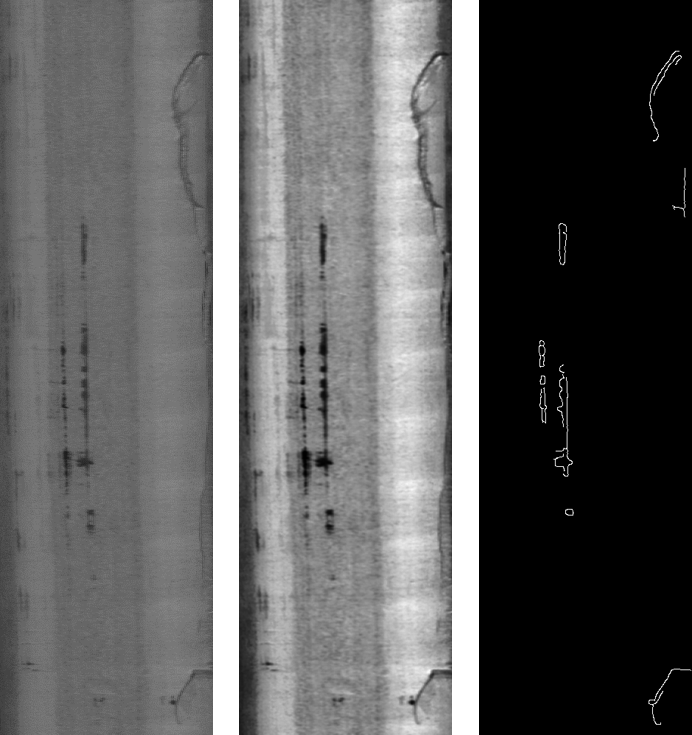
\includegraphics[width=16cm]{c3_edge_detect.png}
    \caption{Canny边缘检测效果图}
    \label{fig:c3_edge_detect}
    \end{figure*}


    \section{形态学操作}
    \esection{Morphology Operation}
    在获取边缘图像之后,需要使用形态学操作\cite{Gonzalez2010Digital,Wilkinson2009Mathematical}将断裂和或者比较接近的边缘连接起来,避免检测的缺陷结果过多。形态学操作是一门以集合论为基础的新兴研究方向,主要被用来分析和描述信号的几何形态。其基本思想是利用设计好的结构元素对信号进行各种形态学处理,能够删除掉不相关的信息,并保留信号的主要形状,作为探针的结构元素可以携带知识,如方向、大小、颜色等信息,不同的结构元素可以得到不同的结果。

    在算法中,主要使用了正方形5x5的形态学算子对边缘图像进行膨胀操作,膨胀会“粗化”二值图像中的物体,用来桥接裂缝。边缘检测出的边缘图像中连通区域较多,可能一个缺陷部分会断裂成多个连通区域,所以膨胀操作用来将这些断裂的情况重新连接起来,接着使用孔洞填充算法填补连通区域内部的孔洞,得到最终的检测结果。

    \section{实验结果}
    \esection{Experimental Results}
        \subsection{数据集与评价方法}
        \esubsection{Data-set and Evaluation Protocol}
        为了验证本方法的有效性,搜集整理了113张带黑斑低对比度缺陷的钢板图像制作了该类缺陷类型测试集,钢板图像的分辨率为289x998,同时为了验证本方法同样适用于其他类型缺陷的检测,搜集整理了125张结疤类型缺陷和100张压痕类型缺陷,并且对每一张缺陷图像都进行了缺陷区域的groundtruth标记,表是对测试集的数据内容总结,图\ref{fig:c3_defect_type} 展示了三种缺陷类型。

        \begin{figure*}[!h]
        \centering
        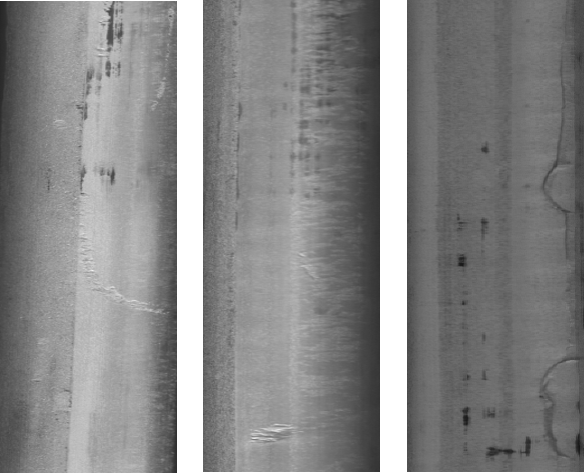
\includegraphics[width=16cm]{c3_defect_type.png}
        \caption{三种不同的缺陷类型,从左至右以及为结疤、压痕和带黑斑低对比度缺陷}
        \label{fig:c3_defect_type}
        \end{figure*}

        \subsection{实验结果与分析}
        \esubsection{Experimental Results and Analysis}
        实验环境为3.10GHZ Intel Core i5,4g内存,win7系统,使用MATLAB和c++代码进行实验。总的检测结果使用以下指标来衡量:查全率、查准率、和F值。

        基于显著性的方法首先对图像进行高斯滤波器进行滤波操作,然后将图像从RGB 空间转换到LAB空间,接着提取出图像的显著性图,然后对显著性图进行canny 边缘检测提取边缘图像,最后对边缘图像进行形态学操作。使用MATLAB 语言实现的部分代码如下:

        \lstinputlisting{code/xianzhuxing.m}

        为了说明本文提出的缺陷检测方法的有效性,使用本文的方法与自适应平滑滤波canny算子检测方法\cite{Canny1986A}以及基于kirsch边缘的缺陷检测方法\cite{李伟2016热态高速线材表面缺陷检测系统研究与实现} 做了对比试验,对于三种缺陷类型的实验结果分别如下表所示:

        \begin{table*}[!h]
        \centering
        \caption{结疤类型缺陷检测结果}
        \label{tbl:c3_salient_result_1}
        \begin{tabularx}{\columnwidth}{>{\centering\arraybackslash}X >{\centering\arraybackslash}X >{\centering\arraybackslash}X >{\centering\arraybackslash}X}
        \toprule
        方法 & 查全率 & 查准率 & F值 \\
        \midrule
        基于显著性图 & 0.9580 & 0.7446 & 0.8382 \\
        Canny边缘检测 & 0.8993 & 0.2487 & 0.3896 \\
        kirsch边缘检测 & 0.7625 & 0.6276 & 0.6885 \\
        \bottomrule
        \end{tabularx}
        \end{table*}

        \begin{table*}[!h]
        \centering
        \caption{压痕类型缺陷检测结果}
        \label{tbl:c3_salient_result_2}
        \begin{tabularx}{\columnwidth}{>{\centering\arraybackslash}X >{\centering\arraybackslash}X >{\centering\arraybackslash}X >{\centering\arraybackslash}X}
        \toprule
        方法 & 查全率 & 查准率 & F值 \\
        \midrule
        基于显著性图 & 0.8803 & 0.7923 & 0.8340 \\
        Canny边缘检测 & 0.8531 & 0.3927 & 0.5378 \\
        kirsch边缘检测 & 0.8536 & 0.6313 & 0.7261 \\
        \bottomrule
        \end{tabularx}
        \end{table*}

        \begin{table*}[!h]
        \centering
        \caption{带黑斑低对比度类型缺陷检测结果}
        \label{tbl:c3_salient_result_3}
        \begin{tabularx}{\columnwidth}{>{\centering\arraybackslash}X >{\centering\arraybackslash}X >{\centering\arraybackslash}X >{\centering\arraybackslash}X}
        \toprule
        方法 & 查全率 & 查准率 & F值 \\
        \midrule
        基于显著性图 & 0.8673 & 0.4959 & 0.6310 \\
        Canny边缘检测 & 0.5877 & 0.2084 & 0.3076 \\
        kirsch边缘检测 & 0.2113 & 0.3987 & 0.2762 \\
        \bottomrule
        \end{tabularx}
        \end{table*}

        实验结果表明在加入了显著性方法之后,对三类缺陷的检测结果均有提升,带黑斑低对比度类型缺陷尤其明显。虽然基于显著性的方法相对于canny算子检测方法对于结疤和压痕两类缺陷的查全率提升并不明显,但是在查准率方面提升很大,这说明在其他两类缺陷中使用原图进行canny边缘检测时,是通过较高的误检率来提高检测缺陷的数量,这在工业生产中仍然会造成相当多的问题,而显著性方法查全率和查准率都较高,整体的性能明显优于单纯使用边缘检测的方法。同时,需要说明的一点是由于带黑斑低对比度图像中存在的黑斑数量过多、灰度值分布范围较广、黑斑形状多变等因素导致黑斑伪缺陷很难被完全滤除,这也导致了实验结果的查全率不是特别高,但是黑斑误检为缺陷的情况已经大幅度降低,相对于其他两种方法的效果已经有了很大的提升。

        在时间方面,自适应平滑滤波canny算子检测方法平均耗时为25ms,基于kirsch 边缘缺陷检测方法平均耗时为18ms,基于显著性的缺陷检测方法平均耗时为40ms,虽然基于显著性的缺陷检测方法相对于其他两种方法的耗时要相对长一些,但是该算法的时间性能已经完全可以满足工业生产的要求了。

        图\ref{fig:c3_salient_result}展示了使用自适应平滑滤波canny算子缺陷检测与基于显著性方法的缺陷检测方法的部分实验结果效果对比,可以看出在使用了改进的显著性检测进行对比度增强和去黑斑之后,检测的缺陷区域更加完整,黑斑伪缺陷的误检大大降低,第二行检测的黑斑区域在第一行中对应的图像中几乎没有检测出来。

        \begin{figure*}[!h]
        \centering
        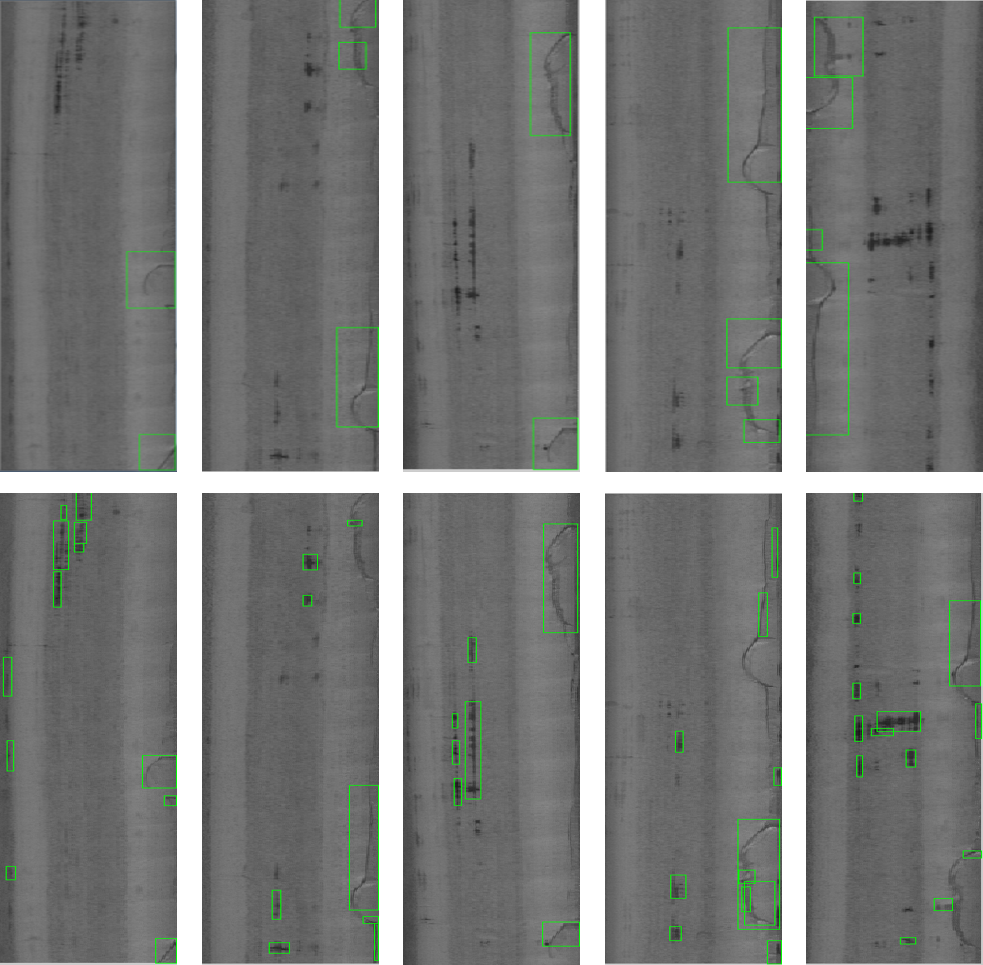
\includegraphics[width=16cm]{c3_salient_result.png}
        \caption{部分检测结果,从上之下依次为基于显著性图的方法和canny算子检测的实验结果}
        \label{fig:c3_salient_result}
        \end{figure*}

        综上实验结果,可以充分说明基于显著性的缺陷检测方法不仅对于低对比度带黑斑缺陷有很好的检测效果,对于其他类型缺陷同样具有良好的检测效果。
    \section{本章小结}
    \esection{Brief Summary}
    本章所提出的基于显著性的缺陷检测方法,很好的解决了目前基于机器视觉的低对比度带黑斑缺陷检测难点,通过该方法,检测出的缺陷更加完整,误检数量明显减少,由于结合了改进的显著性检测方法,去除了图像中黑斑伪缺陷对检测结果的干扰,同时,该方法检测速度快,完全符合缺陷检测中对时间性能的要求。当然,该方法仍有继续研究和改进的空间,如何更加完整的提取到缺陷区域、更加完全的去除黑斑,以及时间性能的进一步提高都将成为接下来的工作重点。

